\documentclass{article}

\usepackage[letterpaper]{geometry}
\usepackage{amsmath}
\usepackage{amssymb}
\usepackage{siunitx}
\usepackage{graphicx}

\title{4125 HW 4}
\author{Duncan Wilkie}
\date{2 March 2022}

\begin{document}

\maketitle

\section*{3.10a}
The heat transfer in this process is, using $\SI{334}{J/g}$ as the latent heat of fusion of water,
\[Q=(\SI{334}{J/g})(\SI{30}{g})=\SI{10}{kJ}\]
The change in entropy is therefore
\[\Delta S=\frac{Q}{T}=\frac{\SI{10}{kJ}}{\SI{273}{K}}=\SI{36.7}{J/K}\]

\section*{3.10b}
The heat capacity of the melted ice cube is $C_{V}=(\SI{4.2}{J/g\cdot K})(\SI{30}{g})=\SI{126}{J/K}$
The change in entropy is therefore, presuming (justifiably) a constant heat capacity,
\[\Delta S=C_{V}\ln\left( \frac{T_{f}}{T_{i}} \right)=(\SI{126}{J/K})\ln\left( \frac{\SI{298}{K}}{\SI{273}{K}} \right)=\SI{137.5}{J/K}\]

\section*{3.10c}
The heat required to melt the ice cube is $C_{V}(\SI{25}{K})=\SI{3150}{J}$
The temoerature of the kitchen doesn't change much, so the change in its entropy is
\[\Delta S=-\frac{Q}{T}=-\frac{\SI{3150}{J}}{\SI{298}{K}}=-\SI{10.6}{J/K}\]
where the negative sign is added because $Q$ is flowing out of the kitchen.

\section*{3.10d}
Adding the changes in entropy,
\[\Delta S_{total}=\SI{137.5}{J/K}-\SI{10.6}{J/K}=\SI{126.9}{J/K}\]

\section*{3.16a}
When the memory was initialized, it is in one of  $2^{2^{33}}$ microstates. For each final state of the system, the previous state could have been any of those initial microstates, so the multiplicity is the above number. The entropy is then
\[S=k\ln\Omega=(\SI{1.38e-23}{J/K})\ln\left( 2^{2^{33}} \right)=\SI{8.22e-14}{J/K}\]

\section*{3.16b}
The corresponding heat would be
\[Q=ST=(\SI{8.22e-14}{J/K})(\SI{300}{K})=\SI{2.56e-11}{J}\]
which is a likely immesurable amount of additional energy.

\section*{3.23}
The expression for the temperature of a two-state paramagnet is
\[\frac{1}{T}=\frac{k}{2\mu B}\ln\left( \frac{N-U/\mu B}{N+U/\mu B} \right)\Leftrightarrow x=\frac{\mu B}{kT}=\frac{1}{2}\ln\left( \frac{N-U/\mu B}{N+U/\mu B} \right)\]
Writing $U/\mu B=N-2N_{\uparrow}$ from\ the definition of $U$,
\[x=\frac{1}{2}\ln\left( \frac{N_{\uparrow}}{N-N_{\uparrow}} \right)=\frac{1}{2}\ln\left( \frac{N_{\uparrow}}{N_{\downarrow}} \right)\]
Plugging this in to the given expression,
\[S=Nk\left[  \ln\left(  2\cosh x\right)-x\tanh x\right]\]\[Nk\left\{\ln\left( 2\cosh\left[ \frac{1}{2}\ln\left( \frac{N_{\uparrow}}{N_{\downarrow}} \right) \right]\right) -\frac{1}{2}\ln\left( \frac{N_{\uparrow}}{N_{\downarrow}} \right)\tanh\left[  \frac{1}{2}\ln\left( \frac{N_{\uparrow}}{N_{\downarrow}} \right)  \right] \right\}\]
\[=Nk\bigg\{ \ln\left( 2\cdot\frac{1}{2}\left[ \frac{\exp\left( \ln\left[ \frac{N_{\uparrow}}{N_{\downarrow}} \right] \right)+1}{\exp\left( \frac{1}{2}\ln\left[ \frac{N_{\uparrow}}{N_{\downarrow}} \right] \right)}\right] \right)\]
\[-\frac{1}{2}\ln\left( \frac{N_{\uparrow}}{N_{\downarrow}} \right)\left[ \frac{\exp\left( \ln\left[ \frac{N_{\uparrow}}{N_{\downarrow}} \right] \right)-1}{\exp\left( \ln\left[ \frac{N_{\uparrow}}{N_{\downarrow}} \right]\right)+1} \right]\bigg\}\]
\[=Nk\left\{ \ln\left( \frac{\frac{N_{\uparrow}}{N_{\downarrow}}+1}{\frac{N_{\uparrow}}{N_{\downarrow}}\sqrt{e}}\right)-\frac{1}{2}\ln\left( \frac{N_{\uparrow}}{N_{\downarrow}} \right)\left[ \frac{\frac{N_{\uparrow}}{N_{\downarrow}}-1}{\frac{N_{\uparrow}}{N_{\downarrow}}+1} \right]\right\}\]
\[=Nk\left\{ \ln(N_{\uparrow}+N_{\downarrow})-\ln(N_{\downarrow})-\ln(N_{\uparrow})+\ln(N_{\downarrow})-\frac{1}{2}-\frac{1}{2}\frac{N_{\uparrow}-N_{\downarrow}}{N_{\uparrow}+N_{\downarrow}}\left( \ln(N_{\uparrow})-\ln(N_{\downarrow}) \right) \right\}\]
\[=Nk\left\{ \ln N - \ln N_{\uparrow}-\frac{1}{2}-\frac{1}{2}\frac{N_{\uparrow}}{N}\ln N_{\uparrow}+\frac{1}{2}\frac{N-N_{\uparrow}}{N}\ln(N-N_{\uparrow})\right\}\]
\[=Nk\ln N-Nk\ln N_{\uparrow}-\frac{N_{\uparrow}}{2}k\ln N_{\uparrow}+\frac{Nk}{2}\ln(N-N_{\uparrow})-\frac{N_{\uparrow}k}{2}\ln(N-N_{\uparrow})-\frac{Nk}{2}\]
Neglecting the merely large terms,
\section*{3.25a}
\[S=k\ln\Omega=k\ln\left[  \left( \frac{q+N}{q} \right)^{q}\left( \frac{q+N}{N} \right)^{N} \right]=k\left[ q\ln(q+N)-q\ln q+N\ln(q+N)-N\ln N\right]\]
\[=k[N\ln N-q\ln q+(q+N)\ln(q+N)]\]
The neglected term is a division of the multiplicity expression by $\sqrt{2\pi q(q+N)/N}$ which, after a logarithm, is asymptotic to $-\log N+\log q+\log(q+N)$ as $q,N\to\infty$ which is $o(N\log N+q\log q+(q+N)\log(q+N))$  in the same limit. It therefore is acceptable to neglect this for large $q$ and $N$.

\section*{3.25b}
Since $U=\epsilon q\Leftrightarrow q=\frac{U}{\epsilon}$, the entropy may be written
\[S=k\left[ N\ln N-\frac{U}{\epsilon}\left(  \ln U-\ln\epsilon\right) +\left( \frac{U}{\epsilon}+N \right)\ln\left( \frac{U}{\epsilon}+N \right)\right]\]
Differentiating with respect to internal energy at constant $N$ and $V$,
\[\frac{1}{kT}=\frac{1}{k}\left( \frac{\partial S}{\partial U} \right)_{N,V}=\frac{\ln\epsilon}{\epsilon}-\left(\frac{1}{\epsilon}+\frac{\ln U}{\epsilon}\right)+\left( \frac{1}{\epsilon}+\frac{1}{\epsilon}\ln\left[ \frac{U}{\epsilon}+N \right]\right)\]
\[\Leftrightarrow T=\frac{\epsilon}{k\ln\left( \frac{U+\epsilon N}{U} \right)}=\frac{\epsilon}{k\ln\left( 1+\frac{\epsilon N}{U} \right)}\]

\section*{3.25c}
Solving for $U$,
\[1+\frac{\epsilon N}{U}=e^{\epsilon/kT}\Leftrightarrow U=\frac{\epsilon N}{e^{\epsilon/kT}-1}\]
Differentiating with respect to temperature,
\[C_{V}=\left(\frac{\partial U}{\partial T}\right)_{N,V}=\frac{\epsilon^{2}Ne^{\epsilon/kT}}{kT^{2}(e^{\epsilon/kT}-1)^{2}}\]

\section*{3.25d}
Using $e^{x}=1+x+O(x^{2})$ as $x\to 0$ and $\frac{1}{T}\to 0$ as $T\to\infty$,
\[C_{V}\approx \frac{\epsilon^{2}N}{k}\frac{1+\frac{\epsilon}{kT}}{T^{2}\left( 1+\frac{\epsilon}{kT}-1\right)^{2}}={k\epsilon^{2}N}\left( \frac{1}{\epsilon^{2}}+\frac{1}{\epsilon k T} \right)\approx Nk\]

\section*{3.25e}

Using gnuplot,
\[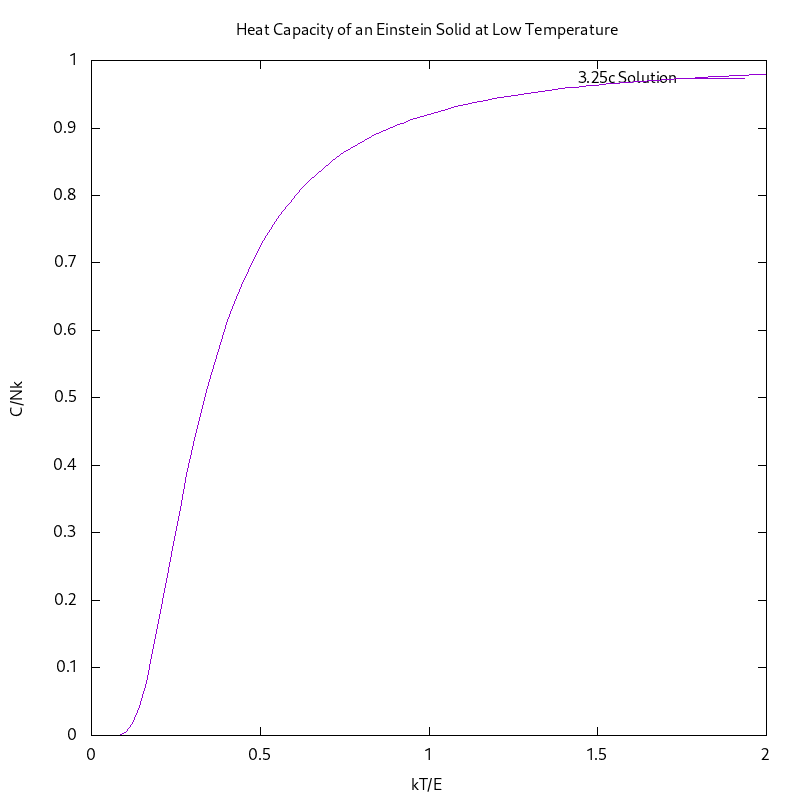
\includegraphics[scale=.7]{cap.png}\]
This predicts an exponential falloff of the heat capacity at low temperature, which is corroborated qualitatively by the experimental data presented in figure 1.14. From this plot, $\frac{kT}{\epsilon}=0.5$ is a little past the inflection point of the curve. Looking at the experimental data, the analogous point is around $\SI{40}{K}$ for lead, $\SI{110}{K}$ for aluminum, and $\SI{400}{K}$ for diamond (the $x$ range of the graph is too short to really tell, but it appears the slope is decreasing at $\SI{400}{K}$, so it's a decent estimate). Solving for $\epsilon$ in the initial equation,
\[\epsilon_{Pb}=2kT_{Pb}=2(\SI{1.38e-23}{J/K})(\SI{40}{K})=\SI{1.1e-21}{J}=\SI{0.0069}{eV}\]
\[\epsilon_{Al}=2kT_{Al}=2(\SI{1.38e-23}{J/K})(\SI{110}{K})=\SI{3.04e-21}{J}=\SI{0.019}{eV}\]
\[\epsilon_{Dia}=2kT_{Dia}=2(\SI{1.38e-23}{J/K})(\SI{400}{K})=\SI{1.10e-20}{J}=\SI{0.069}{eV}\]

\section*{3.25f}
The expression in part (c) up to$x^{3}$ terms is
\[C_{V}\approx \frac{\epsilon^{2}N}{k}\frac{1+\frac{\epsilon}{kT}+\frac{\epsilon^{2}}{2k^{2}T^{2}}+\frac{\epsilon^{3}}{6k^{3}T^{3}}}{T^{2}\left( \frac{\epsilon}{kT}+\frac{\epsilon^{2}}{2k^{2}T^{2}}+\frac{\epsilon^{3}}{6k^{3}T^{3}} \right)^{2}}=\frac{\epsilon^{2}N}{k}\frac{1+\frac{\epsilon}{kT}+\frac{\epsilon^{2}}{2k^{2}T^{2}}+\frac{\epsilon^{3}}{6k^{3}T^{3}}}{T^{2}\left( \frac{\epsilon^{2}}{k^{2}T^{2}}+\frac{\epsilon^{3}}{k^{3}T^{3}}+\frac{\epsilon^{4}}{3k^{4}T^{4}}+ \frac{\epsilon^{4}}{4k^{4}T^{4}}+\frac{\epsilon^{5}}{6k^{5}T^{5}}+\frac{\epsilon^{6}}{36k^{6}T^{6}}\right)}\]
\[=\frac{\epsilon^{2}N}{k}\frac{1+\frac{\epsilon}{kT}+\frac{\epsilon^{2}}{2k^{2}T^{2}}+\frac{\epsilon^{3}}{6k^{3}T^{3}}}{\frac{\epsilon^{2}}{k^{2}}+\frac{\epsilon^{3}}{k^{3}T}+\frac{\epsilon^{4}}{3k^{4}T^{2}}+\frac{\epsilon^{4}}{4k^{4}T^{2}}+\frac{\epsilon^{5}}{6k^{5}T^{3}}+\frac{\epsilon^{6}}{36k^{6}T^{4}}}\]

Call the denominator $p$ for sake of compactness. This becomes
\[=\frac{\epsilon^{2}N}{k}\left( \frac{1}{p}+\frac{\epsilon}{kTp}+\frac{\epsilon^{2}}{2k^{2}T^{2}p} +\frac{\epsilon^{3}}{6k^{3}T^{3}p}\right)\]
The only terms less than $\left(\frac{\epsilon}{kT}\right)^{2} $ are those from the pentultimate summand, so



\section*{3.32a}
The
\end{document}
%%% Local Variables:
%%% mode: latex
%%% TeX-master: t
%%% End:
